% test dokumentu
\documentclass{beamer}
\usepackage{tikz}
\usepackage{hyperref}
\usepackage{multimedia}
\usepackage{graphicx} 
\usepackage[polish]{babel}% Język
\let\babellll\lll
\let\lll\relax% Naprawia błąd \lll
\usepackage{polski}% Język
\usepackage[utf8]{inputenc}% Kodowanie
\usetheme[pagenumbers]{PaloAlto}
\usecolortheme{crane}
\title{Historia internetu}
\subtitle{od A do Z}
\author[Mateusz Szewczak]{Mateusz Szewczak
	\texttt{Politechnika Koszalińska, kierunek Informatyka, grupa I10}}
\date[Koszalin 2020]{06.11.2020}
 \usepackage{wrapfig} 
\begin{document}
	\bibliographystyle{unsrt}
	\begin{frame}
		\maketitle
	\end{frame}
	\begin{frame}{Spis treści}
		\tableofcontents
	\end{frame}
	\begin{frame}{Skąd się wzięła idea sieci}
		\section{Początki internetu}
		\subsection{Jak to się zaczęło?}
		\begin{wrapfigure}{r}{0.5\textwidth}
			\flushright
			\vspace{-30pt}
			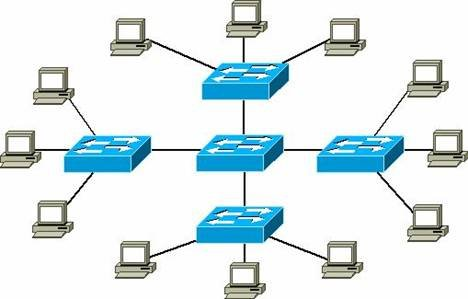
\includegraphics[height=4cm]{gwiazda.jpg}
			\caption{\cite{SOISK.PL}}
		\end{wrapfigure}
		Po~drugiej wojnie światowej USA miała scentralizowaną sieć radiostacji. Potrzebna było rozwiązanie, zapewniające sprawne połączenia w zdecentralizowanej sieci.
		\nocite{hist:int:wiki}
	\end{frame}
	\begin{frame}{Wynalazca}
		\begin{wrapfigure}{r}{0.5\textwidth}
			\flushright
			\vspace{-30pt}
			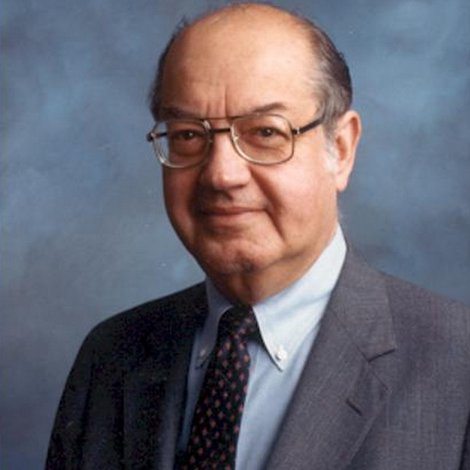
\includegraphics[height=4cm]{baran-zdjecie.jpg}
			\caption{Paul Baran}
		\end{wrapfigure}
		Pomysłodawcą rozwiązania był Paul Baran. \\
		Inżynier, nagrodzony za swoje zasługi wieloma nagrodami.
	\end{frame}
	\begin{frame}{TCP/IP}
		\textbf{TCP/IP} to zespół protokołów, które mają za zadanie znaleźć optymalną drogę wędrówki pakietów oraz dostarczyć wszystkie pakiety do odbiorcy.
	\end{frame}

	\begin{frame}{Bibliografia}
	\section{Bibliografia}
	\bibliography{bibliografia.bib}
	\end{frame}
\end{document}